\chapter{Abbildungen, Tabellen, Quellcode}
\label{chap:Abbildungen}

\section{Allgemeines}

Abbildungen (\emph{figures}) und Tabellen (\emph{tables}) werden üblicherweise
zusammen mit einem nummerierten Titel (\emph{caption}) zentriert
angeordnet (siehe Abb.~\ref{fig:CocaCola}).
Im Text \emph{muss} es zu jeder Abbildung einen Verweis geben und die eigentliche Abbildung
sollte erst \emph{nach} dem ersten Verweis platziert werden.

\begin{figure}
\centering
\includegraphics[width=.95\textwidth]{cola-public-domain-photo-p} %{CS0031}
\caption{Coca-Cola Werbung 1940 \cite{CocaCola1940}.}
\label{fig:CocaCola}
\end{figure}


\section{\emph{Let Them Float!}}

Das Platzieren von Abbildungen und Tabellen gehört zu den
schwierigsten Aufgaben im Schriftsatz, weil diese meist viel Platz
benötigen und häufig nicht auf der aktuellen Seite im laufenden
Text untergebracht werden können. Diese Elemente müssen daher an
eine geeignete Stelle auf nachfolgenden Seiten verschoben werden,
was manuell sehr mühsam (jedoch in \emph{Word} beispielsweise unerlässlich) ist.

In \LaTeX\ funktioniert das weitgehend automatisch, indem
Abbildungen, Tabellen und ähnliche als "Floating Bodies"
behandelt werden. Bei der Positionierung dieser Elemente wird
versucht, einerseits im Textfluss möglichst wenig Leer\-raum
entstehen zu lassen und andererseits die Abbildungen und Tabellen
nicht zu weit von der ursprünglichen Textstelle zu entfernen.

Der Gedanke, dass etwa Abbildungen kaum jemals genau an der
ge\-wünsch\-ten Stelle und möglicherweise nicht einmal auf
derselben Seite Platz finden, ist für viele Anfänger aber offenbar sehr
ungewohnt oder sogar beängstigend. Dennoch sollte man zunächst einmal
getrost \LaTeX\ diese Arbeit überlassen und \emph{nicht} manuell
eingreifen. Erst am Ende, wenn das gesamte Dokument "steht" und
man mit der automatischen Platzierung wirklich nicht zurande
kommt, sollte man (durch gezielte Platzierungsanweisungen
\cite[S.~33]{Oetiker01}) \textbf{in Einzelfällen} eingreifen.



\section{Captions}

Bei Abbildungen steht der Titel üblicherweise \emph{unten}, bei
Tabellen hingegen -- je nach Konvention -- \emph{oben} (wie in diesem Dokument) 
oder ebenfalls \emph{unten}. In \LaTeX\ erfolgt
auch die Nummerierung der Abbildungen automatisch, ebenso der
Eintrag in das (optionale)
Abbildungsverzeichnis%
\footnote{Ein eigenes Verzeichnis der Abbildungen am Anfang des Dokuments
ist zwar leicht erstellt, in einer Diplomarbeit aber (und eigentlich
überall sonst auch) überflüssig. Man sollte es daher weglassen.}
am Beginn des Dokuments.

Die Markierung der Captions%
\footnote{Ausnahmsweise wird das Wort "Caption" im Folgenden
ohne deutsche Übersetzung verwendet.} erfolgt in \LaTeX mithilfe
der \verb!\label{}! Anweisung, die unmittelbar auf die
\verb!\caption{}! Anweisung folgen muss:
%
\begin{lstlisting}[language={[LaTeX]TeX},basicstyle=\small,numbers=left]
\begin{figure}
\centering
\includegraphics[width=.95\textwidth]{cola-public-domain-photo-p}
\caption{Coca-Cola Werbung 1940 \cite{CocaCola1940}.}
\label{fig:CocaCola}
\end{figure}
\end{lstlisting}
%
Der Name des Labels (\texttt{fig:CocaCola}) kann beliebig gewählt werden. 
Die Kennzeichnung \texttt{fig:} ist nur eine nützliche Hilfe, um beim Schreiben verschiedene Arten 
von Labels besser unterscheiden zu können.

Die Länge der Captions kann dabei sehr unterschiedlich sein. Je
nach Anwendung und Stil ergibt sich manchmal eine sehr kurze
Caption (Abb.~\ref{fig:CocaCola}) oder eine längere
(Abb.~\ref{fig:ibm360}).
Man beachte, wie bei kurzen Captions ein
zentrierter Satz und bei langen Captions ein Blocksatz verwendet
wird (\LaTeX\ macht das automatisch).
Captions sollten \emph{immer} mit einem Punkt abgeschlossen sein.%
\footnote{Kurioserweise verlangen manche Anleitungen
genau das Gegenteil, angeblich, weil beim klassischen Bleisatz 
die abschließenden Punkte im Druck häufig "weggebrochen" sind. 
Das kann man glauben oder nicht, im Digitaldruck 
spielt es jedenfalls keine Rolle.}

\begin{figure}
\centering
\includegraphics[width=.85\textwidth]{ibm-360-color}
\caption{Beispiel für einen langen Caption-Text. \textsc{Univac}
brachte 1961 mit dem Modell 751 den ersten Hochleistungsrechner
mit Halbleiterspeicher auf den Markt. Von diesem Computer wurden
in den U.S.A.\ bereits im ersten Produktionsjahr über fünfzig
Exemplare verkauft, vorwiegend an militärische Dienststellen,
Versicherungen und Großbanken. Die Ablöse erfolgte zwei Jahre
später durch das zusammen mit \textsc{Sperry} entwickelte Modell 820.
Das klingt vielleicht plausibel, ist aber völliger Unsinn, denn das
Bild zeigt in Wirklichkeit eine System/360 Anlage von IBM. 
Bildquelle~\cite{IBM360}.} 
\label{fig:ibm360}
\end{figure}




\section{Abbildungen}

Für die Einbindung von Grafiken in \LaTeX\ wird die Verwendung des Stan\-dard-Pakets
\texttt{graphicx} \cite{Carlisle99} empfohlen. 
Mit dem aktuell verwendeten Workflow (\texttt{pdflatex})
können Bild- bzw.\ Grafikformate ausschließlich 
in folgenden Formaten eingebunden werden:
%
\begin{itemize}
	\item \textbf{PNG}: für Grau-, S/W- und Farb-Rasterbilder (bevorzugt),
	\item \textbf{JPEG}: für Fotos (wenn nicht anders vorhanden),
	\item \textbf{PDF}: für Vektorgrafiken (Illustrationen, Strichzeichnungen etc.).
\end{itemize}
%
Bei Rasterbildern sollte wenn möglich PNG verwendet werden, weil die darin 
enthaltenen Bilder verlustfrei komprimiert sind und daher keine sichtbaren Kompressionsartefakte
aufweisen. Im Gegensatz dazu sollte man JPEG nur dann verwenden, wenn das Originalmaterial
(Foto) bereits in dieser Form vorliegt.


\subsection{Wo liegen die Grafikdateien?} 

Die Bilder werden üblicherweise in einem Unterverzeichnis (oder in mehreren Unterverzeichnissen) abgelegt,
im Fall dieses Dokuments in \nolinkurl{images/}.
Dazu dient die folgende Anweisung
am Beginn des Hauptdokuments \nolinkurl{_Diplomarbeit.tex}:
%
\begin{quote}
\verb!\graphicspath{{images/}}!
\end{quote}
%
Der (zum Hauptdokument relative) Pfad \texttt{graphicspath} kann innerhalb des
Dokuments jederzeit geändert werden, was durchaus nützlich ist, wenn man
z.B.\ die Grafiken einzelner Kapitel getrennt in entsprechenden Verzeichnissen
ablegen möchte.
Die Größe der Abbildung im Druck kann durch Vorgabe einer bestimmten
Breite oder Höhe oder eines Skalierungsfaktors gesteuert werden, z.B.:
%
\begin{quote}
\verb!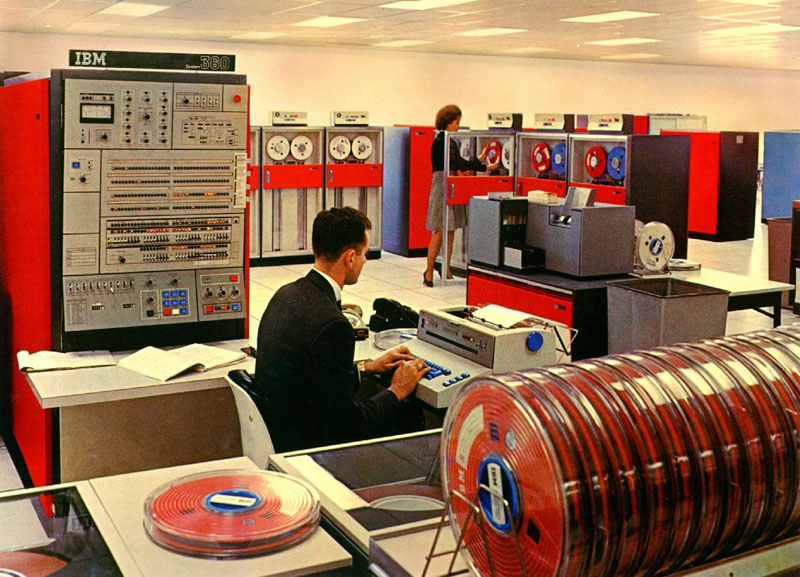
\includegraphics[width=.85\textwidth]{ibm-360-color}! \\
\verb!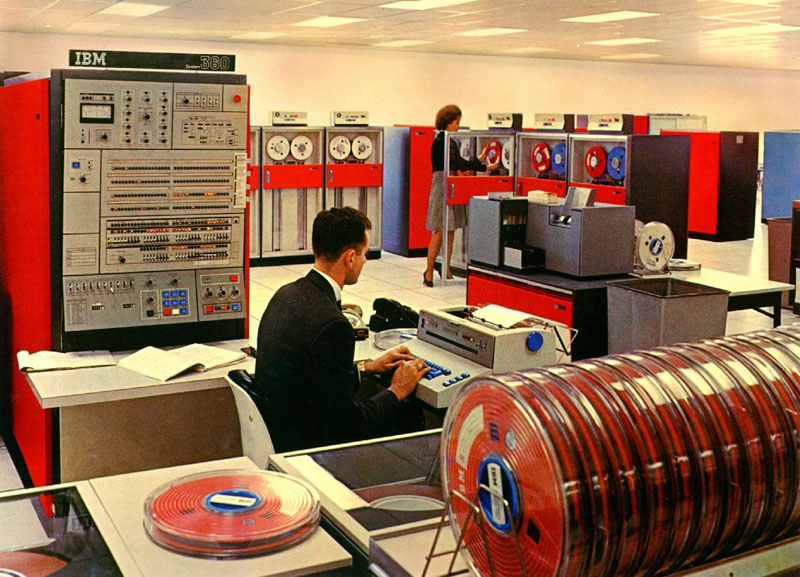
\includegraphics[scale=1.5]{ibm-360-color}!
\end{quote}
%
Man beachte, dass dabei die Dateiendung nicht explizit angegeben werden muss. 
Das ist vor allem dann praktisch, wenn man verschiedene Workflows mit jeweils
unterschiedlichen Dateitypen verwendet.


\subsection{Grafiken einrahmen} 

Mit dem Befehl \verb!\fbox{}! kann man optional einen dünnen 
Rahmen rund um die Grafik erzeugen, z.B.:
%
\begin{quote}
\verb!\fbox{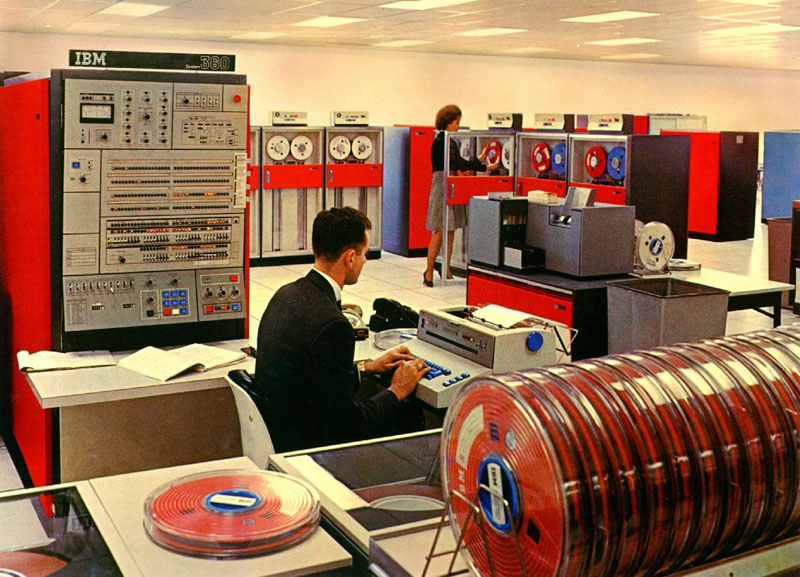
\includegraphics[height=50mm]{ibm-360-color}}!
\end{quote}
%
Das wird man üblicherweise nur bei Rasterbildern tun, insbesondere wenn sie zum Rand hin sehr hell sind
und ohne Rahmen nicht vom Hintergrund abgrenzbar wären.

\subsection{Rasterbilder (Pixelgrafiken)}

Generell sollte man Bilder bereits vorher so aufbereiten,
dass sie später beim Druck möglichst wenig an Qualität verlieren.
Es empfiehlt sich daher, die Bildgröße (Auflösung) bereits im Vorhinein
(z.B. mit \emph{Photoshop})
richtig einzustellen.
Brauchbare Auflösungen bezogen auf die endgültige Bildgröße sind:
%
\begin{itemize}
  \item \textbf{Farb- und Grauwertbilder:} 150--300 dpi
  \item \textbf{Binärbilder (Schwarz/Weiß):} 300--600 dpi
\end{itemize}
%
Eine wesentlich höhere Auflösung macht aufgrund der beim Laserdruck notwendigen
Rasterung keinen Sinn, auch bei 1200 dpi-Druckern.
Speziell \emph{Screen\-shots} sollte man nicht zu klein darstellen,
da sie sonst schlecht lesbar sind (max.\ 200 dpi, besser 150 dpi).
Dabei ist zu bedenken, dass die Arbeit auch als Kopie in allen
Details noch gut lesbar sein sollte.

\subsubsection{JPEG-Problematik}

In der Regel sollte man Bilder, die für den Einsatz in
Druckdokumenten gedacht sind, nicht mit verlustbehafteten
Kompressionsverfahren abspeichern. Insbesondere sollte man die Verwendung
von JPEG möglichst vermeiden, auch wenn viele Dateien dadurch
wesentlich kleiner werden. 
Eine Ausnahme ist, wenn die Originaldaten nur in JPEG vorliegen und für die 
Einbindung nicht bearbeitet oder verkleinert wurden. Ansonsten sollte man immer
PNG verwenden.

Besonders gerne werden farbige \textbf{Screenshots} einer JPEG-Kompression%
\footnote{Das JPEG-Verfahren ist für natürliche Fotos konzipiert und dafür auch gut geeignet,
seine undifferenzierte Verwendung ist aber zu einer globalen Plage geworden.}
unterzogen, obwohl deren verheerende Folgen auch für jeden Laien sichtbar sein sollten
(Abb.~\ref{fig:jpeg-pfusch}).

\begin{figure}
\centering\small
\begin{tabular}{cc}
\fbox{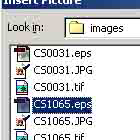
\includegraphics[width=0.45\textwidth]{screenshot-dirty}} &		% JPEG file
\fbox{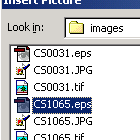
\includegraphics[width=0.45\textwidth]{screenshot-clean}} \\	% PNG file
(a) & (b) 
\end{tabular}
\caption{Typischer JPEG-Pfusch. Screenshots und ähnliche im Original
verfügbare Rasterbilder sollten für Druckdokumente \emph{keinesfalls} mit
JPEG komprimiert werden. Das Ergebnis~(a) sieht gegenüber dem
unkomprimierten Original~(b) nicht nur schmutzig aus, sondern wird
im Druck auch schnell unleserlich.} 
\label{fig:jpeg-pfusch}
\end{figure}






\subsection{Vektorgrafiken}

Für schematische Abbildungen (z.B. Flussdiagramme, Entity-Relationship-Diagramme
oder sonstige strukturelle Darstellungen) sollte man unbedingt
Vektorgrafiken (PDF) verwenden. % (\zB Abb.~\ref{fig:latex-pdf-workflow}).
Gerasterte Grafiken, wie man sie üblicherweise als GIF- oder PNG-Dateien
auf Webseiten findet, haben in einem Druckdokument nichts zu suchen, notfalls
muss man sie mit einem entsprechenden Werkzeug \emph{neu} zeichnen (natürlich
unter Angabe der ursprünglichen Quelle).

In diesem Fall kommt als Datenformat nur PDF %(oder EPS im DVI-PS-Workflow) 
in Frage,
dieses bietet sich aber auch in anderen Umgebungen als universelles
Vektor-Format an.
Zur Erstellung von PDF-Vektorgrafiken benötigt man ein geeignetes
Grafikprogramm, z.B. \emph{Freehand} %von \emph{Macromedia}
oder \emph{Illustrator} von \emph{Adobe}.
Manche gängige Grafikprogramme 
unterstützen allerdings keinen direkten Export von PDF-Dateien
oder erzeugen unsaubere Dateien. Vor der Entscheidung
für eine bestimmte Zeichensoftware sollte man das im Zweifelsfall
ausprobieren.
PDF kann im Notfall über einen entsprechenden Druckertreiber erzeugt werden.




\subsubsection{Einbettung von Schriften}

Die Wiedergabe von Textelementen ist abhängig von der auf dem
Computer (oder Drucker) installierten Schriften und der Form der
Schrifteinbettung im Quelldokument. Die korrekte Darstellung am
Bildschirm eines Computers bedeutet nicht, dass dasselbe Dokument
auf einem anderen Computer oder Drucker genau so dargestellt wird.
Dieser Umstand ist besonders wichtig, wenn Druckdokumente online
zur Verfügung gestellt werden. Kontrollieren Sie daher genau, ob
die innerhalb Ihrer Grafiken verwendeten Schriften auch exakt wie
beabsichtigt im Ausdruck aufscheinen.

